%%%*******************************************************************************
%  Classe Latex UEFS PPGM, Version 1.0.1 13/09/2021
%
%  Define as normas e estilo das dissertações e teses do PPGM-UEFS
%
%  Author : Gilney Zebende
%  Contribuição : João Paulo Just Peixoto <joao.just@ifba.edu.br,just1982@gmail.com>
%%%-------------------------------------------------------------------------------


%%%-------------------------------------------------------------------------------
%  DOCUMENTAÇÃO COM EXEMPLOS
%%%*******************************************************************************

%%%-------------------------------------------------------------------------------
%%% Thesis default options
%%%-------------------------------------------------------------------------------
%\documentclass[subook]{Classes/PPGM-UEFS}
%\documentclass[sureport]{Classes/PPGM-UEFS}

%%%-------------------------------------------------------------------------------
%%% Thesis custom options
%%%-------------------------------------------------------------------------------

%%% Fancy page headings
%\documentclass[fancyheadings, subook]{Classes/PPGM-UEFS}
%\documentclass[fancyheadings, sureport]{Classes/PPGM-UEFS}

%%% Fancy chapters and sections headings
%\documentclass[fancychapter, subook]{Classes/PPGM-UEFS}
%\documentclass[fancychapter, sureport]{Classes/PPGM-UEFS}

%%% Fancy page , chapters and sections headings
%\documentclass[fancyheadings, fancychapter, subook]{Classes/PPGM-UEFS}
\documentclass[fancyheadings, fancychapter, sureport]{Classes/PPGM-UEFS}


%%%-------------------------------------------------------------------------------
%%% Thesis Commands (ONLY with fancy page headings)
%%%-------------------------------------------------------------------------------

%%%Page header line width
%\footlinewidth{value}

%%%Page footer line width
%\headlinewidth{value}

%%%Page header and footer line width
%\headingslinewidth{value}

%%%Page header and footer lines without text
%\headingslinesonly

%%%The default line width is 0.3pt.
%%%Set the value to 0pt to remove the page header and/or footer line

%%%-------------------------------------------------------------------------------
%%% SUThesis Supported Graphic Formats
%%%-------------------------------------------------------------------------------
% The figures formats supported depend upon the selected output file
% Include your figure without the extention, the SUThesis will automatically
% search the predefined `Figures' directory tree for the right file format.
%
% - The pdfLaTEX (PDF) supports graphics inclusions in PDF, JPG, PNG, and
%   MetaPost (with .mps extention) formats.
%
% - The Latex (DVI) supports graphics inclusions in EPS and PS formats.
%%%-------------------------------------------------------------------------------


%%%-------------------------------------------------------------------------------
%%% Árvore de diretório PPGM-UEFS
%%%-------------------------------------------------------------------------------
%  Diretorio
%       \Classes        (requerido)
%       \Figures        (requerido) --------------------------------->
%       \Figures\PDF    (opcional)
%       \Figures\JPG    (opcional) Figuras nestas pastas
%       \Figures\PNG    (opcional) são buscadas automaticamente
%       \Figures\MPS    (opcional) pela classe PPGM-UEFS.
%       \Figures\EPS    (opcional)
%       \Figures\PS     (opcional) <--------------------------------
%       \Tables         (requerido)
%       \Others         (requerido)
%       \Chapters       (requerido)
%       \Appendices     (opcional)
%       \References     (requerido)
%%%-------------------------------------------------------------------------------

%%%-------------------------------------------------------------------------------
%%% Funções auxiliares (não mude isso)
%%%-------------------------------------------------------------------------------
\newcommand{\nth}[2]{
    \foreach \x [count=\k] in #1 {
        \ifnum\k=#2
            \x
        \fi
    }
}

\makeatletter
\newcommand*\ppgmbancalist{}
\newcommand*\ppgmbancaextlist{}
\newcommand*\ppgmbanca[2]{
    \g@addto@macro\ppgmbancalist{{#1,#2},}
}
\newcommand*\ppgmbancaext[2]{
    \g@addto@macro\ppgmbancaextlist{{#1,#2},}
}
\makeatother

% Equações
\newcommand{\dmc}{\(DMC_x^2\) }
\newcommand{\pdcca}{\({\rho}_{DCCA}\) }
\newcommand{\fdfa}{\(F_{DFA}\) }


%%%-------------------------------------------------------------------------------
%%% Dados da tese/dissertação
%%%-------------------------------------------------------------------------------
\newif\ifdoutor
\newif\ifcoor

%% Primeiro indique se é uma tese de doutorado ou dissertação de mestrado:
\doutortrue     % Para tese de doutorado
%\doutorfalse   % Para dissertação de mestrado

%% Indique também se tem co-orientador
\coortrue       % Tenho co-orientador
%\coorfalse     % Não tenho co-orientador



%% Preencha as informações abaixo
\newcommand{\ppgmtitulo}       {\dmc e aprendizado de máquina aplicados à análise de séries temporais de dados meteorológicos}
\newcommand{\ppgmsubtitulo}    {Sub-título da Dissertação ou Tese}
\newcommand{\ppgmautor}        {Fernando Ferraz Ribeiro}
\newcommand{\ppgmorientador}   {Gilney Figueira Zebende}
\newcommand{\ppgmcoorientador} {Juan Alberto Leyva Cruz}
\newcommand{\ppgmcooruniv}     {UNIVERSIDADE ESTADUAL DE FEIRA DE SANTANA} % Instituição do co-orientador
\newcommand{\ppgmpalavraschave}{Séries Temporais, Clima , \dmc, \pdcca, Ciência de Dados, Aprendizado de Máquina}
\newcommand{\ppgmkeywords}     {Time Series, Climate, \dmc, \pdcca, Data Science, Machine Learning}
\newcommand{\ppgmdia}          {15}
\newcommand{\ppgmmes}          {maio}
\newcommand{\ppgmano}          {2023}
\newcommand{\ppgmcidade}       {Feira de Santana, BA}

%% Indique os membros internos da banca (nome e instituição)
% É possível acrescentar membros copiando o comando
\ppgmbanca{Prof. Dr. Fulano}{\ppgmcooruniv}
\ppgmbanca{Profa. Dra. Beltrana}{\ppgmcooruniv}

%% Indique os membros externos da banca (nome e instituição)
\ppgmbancaext{Prof. Dr. Ciclano}{INSTITUTO FEDERAL DA BAHIA}
\ppgmbancaext{Profa. Dra. Fulana}{UNIVERSIDADE FEDERAL DA BAHIA}


%%%-------------------------------------------------------------------------------
%%% Sumário do PDF
%%%-------------------------------------------------------------------------------
\ifdoutor
    \newcommand{\ppgmsubject}{Tese de Doutorado em Modelagem em Ciências da Terra e do Ambiente}
\else
    \newcommand{\ppgmsubject}{Dissertação de Mestrado em Modelagem em Ciências da Terra e do Ambiente}
\fi

\ifpdf
    \hypersetup{backref,
                colorlinks  = true,
                pdftitle    = \ppgmtitulo,
                pdfauthor   = \ppgmautor,
                pdfsubject  = \ppgmsubject,
                pdfcreator  = PPGM-UEFS,
                pdfproducer = PDFLatex,
                pdfkeywords = \ppgmpalavraschave
    }
\fi

%%%-------------------------------------------------------------------------------
%%% Required packages
%%%-------------------------------------------------------------------------------
% - ifthen
% - setspace
% - amsmath
% - amsfonts
% - amssymb
% - amsthm
% - eucal
% - graphics
% - fancyhdr
%%%-------------------------------------------------------------------------------

%%%-------------------------------------------------------------------------------
%%% Optional packages
%%%-------------------------------------------------------------------------------
%\usepackage[latin1]{inputenc}
\usepackage[utf8]{inputenc}
\usepackage{longtable}
\usepackage{multirow}
\usepackage{lscape}
\usepackage{graphicx}
\usepackage{float,subfigure}
\usepackage{cite}
\usepackage{tikz}
\usepackage{algorithm}
\usepackage{algorithmic}
\usepackage{listings}
\usepackage{lipsum}

%\usepackage{abntex2cite}
\usepackage[alf]{abntex2cite}

\usepackage[left=3cm,top=3cm,right=2cm,bottom=2cm]{geometry}
\usepackage{ifpdf}
% Tables and Figures Caption
\setlength{\LTcapwidth}{\textwidth}

%\newtheorem{theorem}{Teorema}
%\newtheorem{definition}[theorem]{Defini\c{c}\~ao}

\usepackage{hyperref}

% Traduz os títulos dos algoritmos
\makeatletter
\renewcommand{\ALG@name}{Algoritmo}
\renewcommand{\listalgorithmname}{Lista de  \ALG@name s}
\renewcommand{\algorithmicrequire}{\textbf{Entrada:}}
\renewcommand{\algorithmicensure}{\textbf{Saída:}}
\makeatother

%%%-------------------------------------------------------------------------------
%%% Documento raiz da tese/dissertação
%%%-------------------------------------------------------------------------------
\begin{document}
    %%----------------------------------------------------------------------------
    %% Página de título
    %%----------------------------------------------------------------------------
    % Informações da capa. Não é preciso mudar nada aqui.
    \university{UNIVERSIDADE ESTADUAL DE FEIRA DE SANTANA}
    \faculty{Programa de Pós-graduação em Modelagem em Ciências da Terra e do Ambiente}
    
    \ifdoutor
        \course{Doutorado em Modelagem em Ciências da Terra e do Ambiente}
        \typework{Tese de doutorado}
        \thesisdegreetitle{Doutor em Modelagem em Ciências Ambientais}
    \else
        \course{Mestrado em Modelagem em Ciências da Terra e do Ambiente}
        \typework{Dissertação de Mestrado}
        \thesisdegreetitle{Mestre em Ciências Ambientais}
    \fi
    
    \thesistitle{\ppgmtitulo}
    \hidevolume
    \thesisvolume{Volume 1 de 1}
    \thesisauthor{\ppgmautor}
    \thesisadvisor{\ppgmorientador}
    \ifcoor
        % Caso não queira exibir o nome do(a) co-orientador(a), habilite a linha abaixo:
        %\hidecoadvisor 
        \thesiscoadvisor{\ppgmcoorientador}
    \fi
    \thesismonthyear{\ppgmmes\space de \ppgmano}
    \maketitlepage

    %%----------------------------------------------------------------------------
    %% Inserir Folha de rosto, Nota de estilo, folha de assinaturas, dedicatória
    %%----------------------------------------------------------------------------
    % Comente qualquer linha que não queira inserir
    %==========================================================
%        Document: PPGM-UEFS
%        File....: FolhaRosto.TEX
%        Author..: Gilney Zebende, João Paulo Just Peixoto
%        Date....: 13 de setembro de 2021
%==========================================================
\begin{folharosto}

\begin{center}
\theauthor
\end{center}
\ \\
\ \\
\ \\
\ \\
\ \\
\begin{spacing}{2}
   \begin{center}
   {\LARGE {\bf \thetitle}}
   \end{center}
\end{spacing}
\ \\
\ \\
\ \\
\begin{flushright}

   \begin{list}{}{
      \setlength{\leftmargin}{4.5cm}
      \setlength{\rightmargin}{0cm}
      \setlength{\labelwidth}{0pt}
      \setlength{\labelsep}{\leftmargin}}

      \item \thetypework apresentada ao \thefaculty, Curso de \thecourse
      da \theuniversity, como requisito parcial para a obtenção do
      título de {\bf \thedegreetitle}.

    \begin{list}{}{
      \setlength{\leftmargin}{0cm}
      \setlength{\rightmargin}{0cm}
      \setlength{\labelwidth}{0pt}
      \setlength{\labelsep}{\leftmargin}}

      \item Área de conhecimento: Estudos Ambientais e Geotecnologias

      \item Orientador: Dr. \theadvisor
      \newline \hspace*{2.1cm}  {\footnotesize {\it \theuniversity}}
      
      \ifcoor
          \item Co-orientador: Dr. \thecoadvisor
          \newline \hspace*{2.1cm}  {\footnotesize \emph{\ppgmcooruniv}}
      \fi
      \end{list}
   \end{list}

\end{flushright}

\vspace*{\fill}

%\begin{spacing}{1.5}
   \begin{center}
   \ppgmcidade \par
   \theuniversity \par
   \ppgmano
   \end{center}
%\end{spacing}

\end{folharosto}

    %==========================================================
%        Document: PPGM-UEFS
%        File....: NotaEstilo.TEX
%        Author..: Gilney Zebende
%        Date....: 24 de abril de 2018
%==========================================================

\begin{notaestilo}
Esta \thetypeworkthree foi elaborada considerando as normas de estilo propostas e aprovadas pelo colegiado do \thefacultytwo e est\~ao dispon\'iveis no formato eletr\^onico (\url{http://ppgm.uefs.br/banco-de-dissertacoes}) ou no formato impresso para consulta. \\


\end{notaestilo}

    %==========================================================
%        Document: PPGM-UEFS
%        File....: FolhaAssinaturas.TEX
%        Author..: Gilney Zebende, João Paulo Just Peixoto
%        Date....: 14 de setembro de 2021
%==========================================================

\begin{folhaassinaturas}

%\thispagestyle{empty}

\def\signature#1#2{\parbox[b]{1in}{\smash{#1}\vskip12pt}
\hfill \parbox[t]{4in}{\shortstack{\vrule width 4in height
0.4pt\\\small#2}}}

\def\InstituicaoMembro#1#2{\parbox[b]{1in}{\smash{#1}\vskip12pt}
\hfill \parbox[t]{4in}{\shortstack{\vrule width 4in \\\small#2}}}

\def\signaturepage{%

    \begin{spacing}{1.5}
        \begin{center}
        {\LARGE \theuniversity} \\
        {\large \thefaculty} \\
        {\large \thecourse} \\
        \end{center}
    \end{spacing}

   \vskip 0.25in plus 0.4in minus 0.1in

    \begin{spacing}{1.0}
        \begin{sloppypar}
        A Banca Examinadora, constitu\'ida pelos professores listados abaixo, leu e recomenda a aprova\c{c}\~ao da
        \thetypeworktwo, intitulada ``\thetitle'',
        apresentada no dia (dia) de (m\^es) de (ano), como requisito
        parcial para a obten\c{c}\~ao do t\'itulo de {\bf \thedegreetitle}.\\
        \end{sloppypar}
    \end{spacing}

    \def\sigskip{\vskip0.15in plus 0.2in minus 0.1in}
    \def\beginskip{\vskip0.3875in plus 0.2in minus 0.1in}

    \beginskip
    \signature{Orientador:}{ \theadvisor} \\
    \InstituicaoMembro{}{\theuniversity} \\

    \ifcoor
        \sigskip
        \beginskip
        \signature{Co-Orientador:}{ \thecoadvisor} \\
        \InstituicaoMembro{}{\ppgmcooruniv} \\
    \fi

    \foreach \i in \ppgmbancaextlist {
        \ifx\i\empty{}
        \else
            \sigskip
            \beginskip
            \signature{Membro externo da Banca:}{\nth{\i}{1}} \\
            \InstituicaoMembro{}{\nth{\i}{2}} \\
        \fi
    }
    
    \foreach \i in \ppgmbancalist {
        \ifx\i\empty{}
        \else
            \sigskip
            \beginskip
            \signature{Membro interno da Banca:}{\nth{\i}{1}} \\
            \InstituicaoMembro{}{\nth{\i}{2}} \\
        \fi
    }

    \vfill
    \newpage
    \setcounter{page}{3}
}
%*********************************************************************


\signaturepage


\end{folhaassinaturas}

    %==========================================================
%        Document: PPGM-UEFS
%        File....: Dedicatoria.TEX
%        Author..: Gilney Zebende, João Paulo Just Peixoto
%        Date....: 14 de setembro de 2021
%==========================================================

\begin{dedicatoria}
%\thispagestyle{empty}

\vspace*{\fill}

\begin{flushright}
Dedico este trabalho a...
\end{flushright}
\end{dedicatoria}

    %==========================================================
%        Document: PPGM-UEFS
%        File....: Agradecimentos.TEX
%        Author..: Gilney Zebende
%        Date....: 24 de abril de 2018
%==========================================================
% Neste arquivo de agradecimentos é preciso usar \\ para saltar parágrafos.

\begin{agradecimentos}

\ \\
Ao Prof. Dr. \theadvisor, pela orientação e dedicação ao tema escolhido, e por ter acreditado na pesquisa .\\
\\
Ao Prof. Dr. \thecoadvisor \\
\\
A UEFS e ao PPGM pelos recursos proporcionados para a elaboração da pesquisa\\
\\

\noindent
\ppgmcidade, Brasil \hfill \theauthor\\
\ppgmdia\space de \ppgmmes\space de \ppgmano
\end{agradecimentos}


    %%----------------------------------------------------------------------------
    %% Resumo/abstract, sumário e siglas
    %%----------------------------------------------------------------------------
    % Comente qualquer linha que não queira inserir
    \begin{romanpagenumbers}
        % Resumo e abstract
        \begin{thesisresumo}

Escreva aqui o seu resumo em português.\\

\textbf{Palavras Chaves:} \ppgmpalavraschave

\end{thesisresumo}

        \begin{thesisabastract}

Write here your abstract in english.\\

\textbf{Keywords:} \ppgmkeywords

\end{thesisabastract}

        
        % Sumários
        \thesiscontents
        
        % Lista de quadros (remova se seu texto não possuir quadros)
        \listofquadro
        
        % Lista de algoritmos (remova se seu texto não possuir algoritmos)
        \listofalgorithms
        
        % Abreviações
        \begin{thesisabbreviations}
\begin{footnotesize}
\begin{longtable}[l]{p{2cm}l}

    %%% Lista de siglas e abreviações
    % Faça conforme o modelo:
    %
    % SIGLA \dotfill & Descrição da sigla \\
    UEFS    \dotfill & Universidade Estadual de Feira de Santana \\
    PPGM    \dotfill & Programa de Pós-Graduação em Modelagem em Ciências da Terra e do Ambiente \\
    CAPES   \dotfill & Coordenação de Aprefeiçoamento de Pessoal de Nível Superior \\
    DCCA    \dotfill & \emph{Detrended Cross-Correlation Analysis} \\
    DFA     \dotfill & \emph{Detrended Fluctuation Analysis} \\
    \dmc     \dotfill & \emph{Detrended Multiple Cross-Correlation Coefficient} \\
    \pdcca  \dotfill & \emph{Detrended Cross-Correlation Coefficient}

\end{longtable}
\end{footnotesize}
\end{thesisabbreviations}


        % Volta à numeração de página padrão
    \end{romanpagenumbers}

    %%----------------------------------------------------------------------------
    %% Inclui capítulos da tese/dissertação
    %%----------------------------------------------------------------------------
    \parskip=\baselineskip
    % Comente qualquer linha que não queira inserir
    \chapter{Introdução}
\label{cap:introducao}


\begin{flushright}
``Ordinary life is pretty complex stuff.''\\
(Harvey Pekar)
\end{flushright}

Os sistemas complexos compreendem um campo interdisciplinar da ciência que não possui uma definição exata. Este campo procura estudar numericamente um conjunto amplo de fenômenos não determinísticos, formados pela contribuição de um conjunto (geralmente grande) de componentes (muitas vezes simples) que, interagindo, estruturam-se de forma auto-organizada, gerando resultados inesperados, que não podem ser previstos pelos estudos estatísticos e/ou matemáticos tradicionais dos elementos formadores do sistema.

Na área dos estudos ambientais, os sistemas complexos possuem diversas aplicações: sistemas de transportes, redes de energia e comunicação, organizações sociais e econômicas, densidade e ocupação humana do espaço, dentre outas. Os estudos do clima ocupam um espaço de particular relevância na intercessão entre os estudos ambientais e os sistemas complexos. Em 2021 a Academia Real das Ciências da Suécia concedeu metade do Prêmio Nobel de Física para Syukuro Manabe e Klaus Hasselmann, cujos estudos apresentam modelos complexos para a análise do clima. Em particular apontam uma correlação entre as emissões de dióxido de carbono e as mudanças climáticas.

A aquisição, manipulação, gestão, armazenamento e criação de valor a partir de dados, através de ambientes computacionais, tem-se apresentado como um novo paradigma tecnológico. Um campo do conhecimento que recebeu a denominação de Ciência de Dados, conceito que envelopa alguns termos frequentemente associados à inovação científica, técnica e social como \emph{Big Data}, mineração de dados, \emph{Business Intelligence} internet das coisas, inteligência artificial e aprendizado de máquina(AM), dentre outros \cite[p. 12-13]{EMCdata2015}.

As séries temporais são definidas como um conjunto de observações (numéricas ou categóricas) ordenado no tempo.  Embora muitos dos dados que descrevem as dinâmicas espaciais podem ser registrados na forma de sérias temporais (abastecimento de água nas tubulações, consumo de energia elétrica nos imóveis, fluxos de pessoas e veículos pela cidade, casos de uma doença por dia, etc.), contudo as técnicas de medição de correlações, bem como a devida exploração destas para inferir novos conhecimentos, permanecem como perguntas abertas em muitas sub-áreas das ciências ambientais\cite{Bermudez-Edo2018}.


\section{Definição do problema}
\label{sec:problema}

Os fenômenos climáticos apresentam as características dos sistemas complexos. Um sistema integrado, envolvendo aspectos globais e as condicionantes planetárias, fatores locais de cobertura da terra, proximidade de corpos d'agua, regime de ventos, dentre outros. Em alguns casos, podendo citar o bioma dominante de um determinado lugar, o fator tanto influencia o clima quanto é influenciado por ele.

As inter-relações entre as diversas variáveis climáticas não podem ser facilmente correlacionadas em grande escala. É possível estabelecer relações entre certas medidas meteorológicas em uma determinada localidade, ainda que as relações entre essas não sejam necessariamente relações que podem ser transportadas para toda e qualquer localidade do planeta. Mas a possibilidade de estabelecer relações em rede entre as variáveis climáticas de diferentes localidades umas com as outras ainda é um problema aberto.

\section{Importância da Pesquisa}
\label{sec:justificativa}



\section{Limites e Limitações}
\label{sec:limites}


\section{Questões e Hipóteses}
\label{sec:questoes}

É possível estabelecer e medir correlações entre aspectos climáticos de uma determinada localidade e um conjunto de outras localidades?

A hipótese é de que os fenômenos climáticos estão relacionados e forma complexa. Massas de ar percorrem distâncias na atmosfera, 

\section{Aspectos Metodológicos}
\label{sec:metodologia}


\section{Organização da Tese}
\label{sec:organizacao}

    \chapter{Fundamentação Teórica}
\label{cap:fund_teorica}

\section{Métodos de Análise de Séries Temporais}
\label{sec:dmc}

O coeficiente \pdcca~\cite{Zebende2011} foi formulado tendo como bases o \emph{Detrended Fluctuation Analysis} (DFA)~\cite{Peng_1994} e o \emph{Detrended Cross-Correlation Analysis} (DCCA)~\cite{Podobnik2008}. O DFA é um método de análise de uma série temporal que fornece um parâmetro de auto-afinidade. O termo \emph{Detrended} refere-se a eliminação de uma tendência. O processo é executado em 6 passos:

\begin{enumerate}
    \label{dfa}
    \item Pegando a série temporal \(\{x_{i}\}\) com  \(i\) variando de  \(1\) à \(N\), a série integrada \(X_{k}\) é calculada por \(X_{k} = \sum_{i=1}^{k}\left[x_{i} - \langle x \rangle \right] \) com \(k\) também variando entre \(1\) e \(N\);
    \item A série  \(X_{k}\) e dividida em \(N - n\) caixas de tamanha\(n\) (escala temporal), cada caixa contendo \(n + 1\) observações, iniciando em \(i\) até \(i + n\);
    \item Para cada caixa um polinômio (geralmente de grau 1) é ajustado, gerando \(\widetilde{X}_{k, i}\) with \( i \le k \le (i + n) \) eliminando assim a tendência (detrended values);
    \item  para cada caixa é calculado: \(f_{DFA}^{2}(n, i) = \frac{1}{1+n} \sum_{k=i}^{i + n}(X_{k}-\widetilde{X}_{k, i})^{2}\)
    \item Para todas as caixas de umaescala temporal o DFA é calculado como: \(F_{DFA}(n) = \sqrt{\frac{1}{N - n} \sum_{i=1}^{N-n} f_{DFA}^{2}(n, i)}\);
    \item Para um número de diferentes escalas temorais (n), com valores possíveis entre \( 4 \le n \le \frac{N}{4}\), a função \(F_{DFA}\) é calculada para encontrar a relação entre \(F_{DFA} \times n\)
  \end{enumerate}

DFA também  representa as propriedades de auto-correlação de longo alcance de uma lei de potência~\cite{Zebende2013}. Se a correlação não existe, ou é uma correlação de curto alcance o valor do parâmetro \(\alpha = 0.5\), \(\alpha < 0.5\) indica antipersistência e \(\alpha > 0.5\) persistência.

O \(DCCA\) generaliza o DFA para estabelecer a correlação entre duas séries temporais \cite{Podobnik2008}. O valor deste coeficiente tende a ser a média dos valores do DFA das duas séries. 

Este coeficiente \(\lambda\) indica a existência de uma correlação entre duas séries regidas por leis de potência, mas não quantifica o nível desta correlação. O \emph{Detrended cross-correlation coefficient} ou \pdcca (equação \ref{eq_pdcca}) é um coeficiente que, variando entre -1 e 1, aponta ausência de correlação cruzada para valores próximos de zero, sendo maior a correlação quanto mais o valor se aproximar de 1 e maior a antecorrelação quanto mais o valor se aproximar de -1~\cite{Zebende2011}. 

\begin{equation}
\label{eq_pdcca}
\rho DCCA(n) = \frac{F_{DCCA}^2 (n)}{ F_{DFA1} (n) F_{DFA2} (n)}
\end{equation}

O método foi estatisticamente validado~\cite{PhysRevE.84.066118}, testado~\cite{vassolerZebende2012, Guedes2017, Ferreira2018},
e critérios para avaliação de relevância estatísticas do resultados foram desenvolvidos~\cite{Guedes2018,Guedes2018a}.

O \pdcca~foi estendido para calcular a correlação cruzada de múltiplas series temporais. Denominado \emph{Detrended Multiple Cross-Correlation Coefficient}~(\dmc), representa a generalização do \pdcca para múltiplas variáveis~\cite{Zebende2018}. Implementado com abordagem de janelas móveis~\cite{Guedes2021} e foi desenvolvido um teste estatístico para o coeficiente múltiplo~\cite{DaSilvaFilho2021}

Já que muitos dos problemas que envolvem sistemas complexos lidam com mais de uma variável independente. E os sistemas e AM costumam abordar múltiplas variáveis independentes em suas buscas por padrões, dentre os métodos correlatos ao \pdcca, o \dmc apresenta as qualidades mais promissoras para embasar um algoritmo de AM.

\section{Aprendizado de Máquina e Redes Neurais Artificiais}
\label{sec:ml}

O aprendizado de máquina consiste na aplicação de algoritmos capazes de, através do processamento de um grande conjunto de dados, encontrar padrões, generalizar os critérios de encontrar padrões e prever eventos futuros\cite{bendavid2014}.

\begin{figure}[!htb]
	\centering
	\caption{Aprendizado de Máquina- diagrama conceitual}
	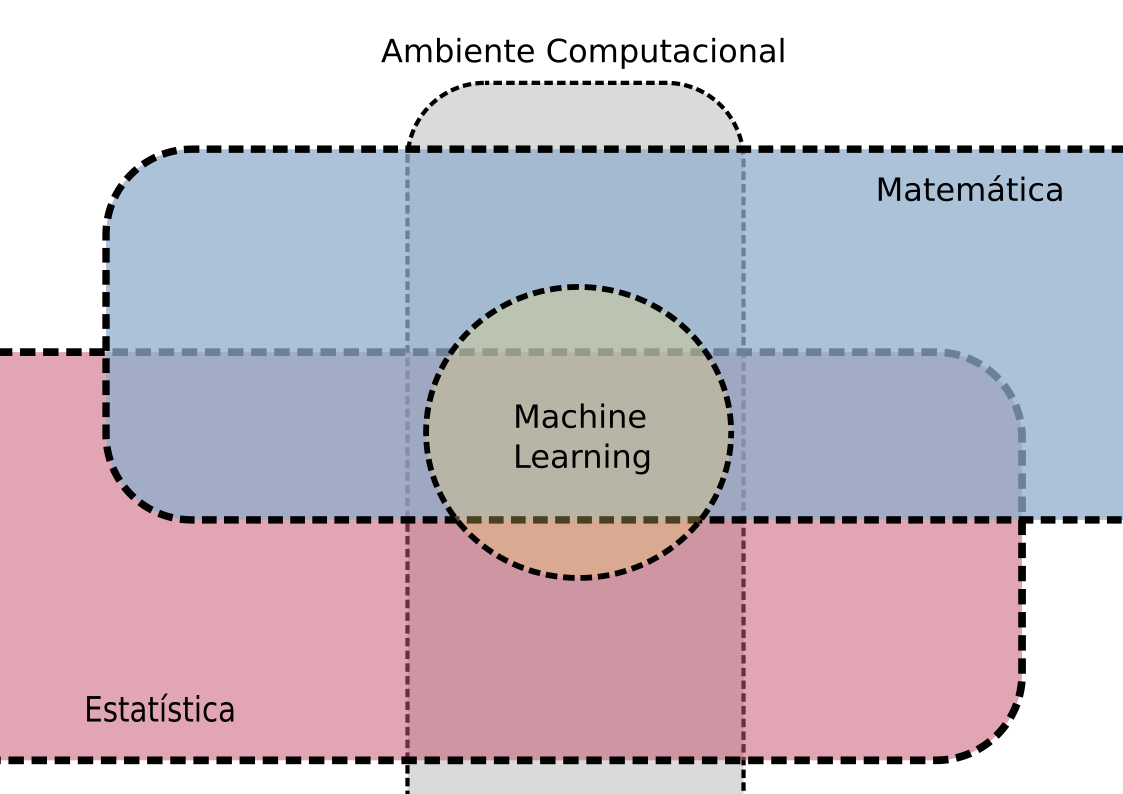
\includegraphics[width=.7\textwidth]{../Figures/ML/mat_est_ML.png}
	\\{\footnotesize Fonte: Elaborada Pelos Autores}
	\label{fig:MLdiag}
\end{figure}

Um campo guiado pela experimentação prática \cite{bishop2006}, pode ser definido pela busca em melhorar o desempenho computacional na realização de uma tarefa, através da experiência \cite{mitchell1997}. O desempenho nesta definição refere-se principalmente a quantificação dos acertos de acordo com uma métrica adequada à resolução do problema em questão e a experiência refere-se a um conjunto de dados coletados.

As tarefas em que os métodos de ML costumam superar os outros algoritmos também apresentam características peculiares: tratam de problemas fracamente definidos do ponto de vista matemático e/ou cujos métodos de resolução matemática são muito custosos do ponto de vista computacional em relação à velocidade necessária para a solução do problema na prática.

Reconhecimento facial e outras formas de interpretação de imagens, máquinas que andam, nadam e dirigem veículos, processamento de linguagem natural (falada e escrita) são exemplos de problemas fracamente definidos. Como definir com instruções de programação convencionais a sequência de instruções necessárias para ensinar um computador a resolver um dos destes problemas? Os algoritmos de ML tem apresentado boas respostas para este tipo de problema.


    \chapter{Metodologia}
\label{cap:metodologia}

    \chapter{Conclusões}
\label{cap:conclusao}

    % Caso precise de mais capítulos, basta criar novos arquivos e acrescentá-los
    % aqui seguindo o modelo acima

    %%----------------------------------------------------------------------------
    %% Inclui anexos
    %%----------------------------------------------------------------------------
    % Comente qualquer linha que não queira inserir
    \begin{thesisappendices}
        \chapter{Anexo I}
\label{anex1}
\begin{center}
    \textbf{Aqui pode ser um Título do seu Anexo}
\end{center}

Texto do Anexo.

        % Caso precise de mais anexos, basta criar novos arquivos e acrescentá-los
        % aqui seguindo o modelo acima
    \end{thesisappendices}

    %%----------------------------------------------------------------------------
    %% Configurar as referencias bibliográficas
    %%----------------------------------------------------------------------------
    \addcontentsline{toc}{chapter}{Referências}
    %\bibliographystyle{abntex2}
    %\bibliographystyle{unsrt}
    %\bibliographystyle{abnt}
    \bibliography{References/referencias}
    
    %%----------------------------------------------------------------------------
    %% Finalização
    %%----------------------------------------------------------------------------
    %==========================================================
%        Document: PPGM-UEFS
%        File....: UltimaFolha.TEX
%        Author..: Gilney Zebende
%        Date....: 24 de abril de 2018
%==========================================================
\begin{ultimafolha}

\vspace*{\fill}

\begin{flushleft}
{\it \thetitle} \\
\ \\
\theauthor \\
\ \\
\ppgmcidade, \ppgmmes\space de \ppgmano.
\end{flushleft}
\end{ultimafolha}

\end{document}

%%%-------------------------------------------------------------------------------
%%% Aqui finalizamos a formatação. Faça um bom trabalho.
%%%-------------------------------------------------------------------------------
